\section{Spørgsmål 7}

% Structured Query Language SQL, herunder begreberne DML og DDL, samt strukturen for og mulighederne med de forskellige typer SQL erklæringer.

\subsection{Fokuspunkter}
\begin{itemize}
	\item Structured Query Language SQL.
	\begin{itemize}
		\item Herunder begreberne DML og DDL.
		\item Samt strukturen for og mulighederne med de forskellige typer SQL erklæringer
	\end{itemize}
\end{itemize}

\subsection{Litteratur}
\begin{itemize}
	
	\item Fra teori: Database Modeling and Design. Logical Design 5'th Ed.
	\begin{itemize}
		\item Appendix "The Basics of SQL" page 261-277.
	\end{itemize}
	
	\item Fra Database eLearning: \url{http://db.grussell.org/index.html}.
	\begin{itemize}
		\item Ch. 3 SQL
		\begin{itemize}
			\item Simple SELECT statements.
			\item Logical Operators and Aggregation.
			\item JOINs and VIEWs.
			\item Subqueries and Schema.
			\item Order of Evaluation.
		\end{itemize}
	\end{itemize}
	
%	\item Fra wikipedia:
%	\begin{itemize}
%		\item 
%	\end{itemize}
%	
%	\item Fra Agile Data Home Page:
%	\begin{itemize}
%		\item 
%	\end{itemize}
\end{itemize}

\newpage

% must
\subsection{Structured Query Language SQL}
SQL er er special purpose sprog der bruges til at manage relationelle databaser.

SQL består af 3 moduler.

\textbf{DML - Data Manipulation Language}
\textbf{DDS - Data Definition Language}
\textbf{Data Control Language}

\subsubsection{Elementer i sproget}

\begin{itemize}
	\item Clauses: UPDATE, SET, WHERE osv.
	\item Expressions: X+1.
	\item Statements: X = X+1.
	\item Predicates: X = 'Y'
	\item Operators: Minder meget om standar C operatorer. Afvigelser og specielle SQL operatorer har vi følgende:
	\begin{itemize}
		\item $!=$ er i SQL $<>$
		\item BETWEEN - Eksempel \textbf{Cost BETWEEN X AND Y}
		\item LIKE - Match af nogen dele af en parameter. Eksempel \textbf{Name LIKE 'Hans'}
		\item IN - Lig med en eller flere parametre. Eksempel \textbf{Number IN (1,6,5)}
		\item IS eller IS NOT - Eksempel \textbf{Name IS NOT NULL}
		\item IS NOT DISTINCT FROM - dunno.
		\item AS - Ændre et fieldname ved visning. Eksempel \textbf{SELECT Name AS 'Navn'}
	\end{itemize}
	\item Statement terminator ;
	
\end{itemize}

\begin{figure}
\centering
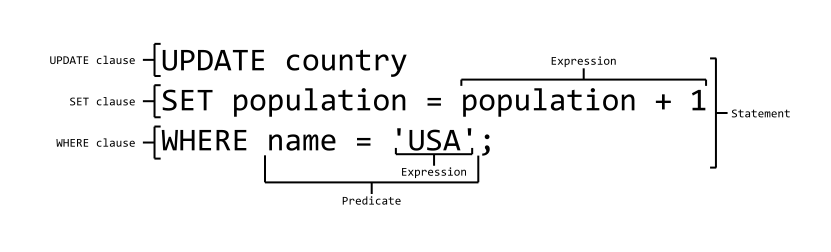
\includegraphics[width=0.9\linewidth]{figs/spm7/sqlDecomp}
\caption{Elemter i SQL}
\label{fig:sqlDecomp}
\end{figure}

% must
\subsubsection{Herunder begreberne DML og DDL}

\paragraph{DML}
DML er en syntaks samling der gør det muligt at manipulere data i en database.
DML bruges når vi vil arbejde med den data som allerede eksisterer i databasen, herunder lave Queries, Sub-queries, Insertions, Opdateringer, Sletninger og Merges.



\paragraph{DDL}

% must
\subsection{Samt strukturen for og mulighederne med de forskellige typer SQL erklæringer}

\subsubsection{Statement struktur}

\subsubsection{Muligheder med SQL statements}

\begin{itemize}
	\item Data Definition - CREATE, DROP, ALTER
	\item Queries og Sub-Queries - SELECT, JOIN
	\item Data manipulation - INSERT, UPDATE, DELETE og MERGE
\end{itemize}